Segmentation of white powders by Specim Scanner in infrared wavelengths is operated in two ways.

First method is to use the selected areas for segmentation. The selected areas and results are shown in Figure \ref{fig:powder-specim-ir-1}. 

The codes for this task can be found in Code \ref{code:powder}. The functions in the code are imported from the Code \ref{code:segmentation}.

\begin{figure}[H]
  \centering
  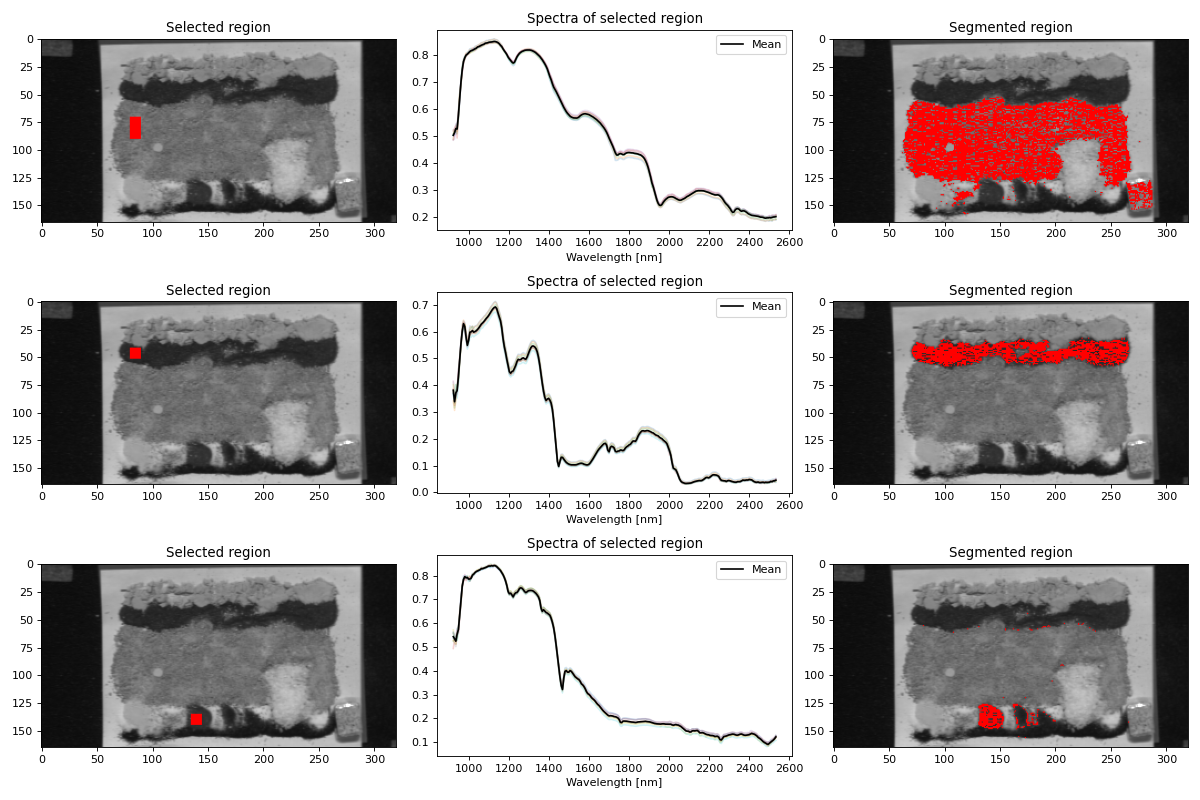
\includegraphics[width=0.8\textwidth]{./fig/task3/powder.png}
  \caption{Selected areas for segmentation by Specim Scanner in infrared wavelengths}
  \label{fig:powder}
\end{figure}

Second method is to use RGB visualization of the spectral image. The segmentation results are shown in Figure \ref{fig:powder-seg}

The codes for this task can be found in Code \ref{code:powder-segment}.

\begin{figure}[H]
  \centering
  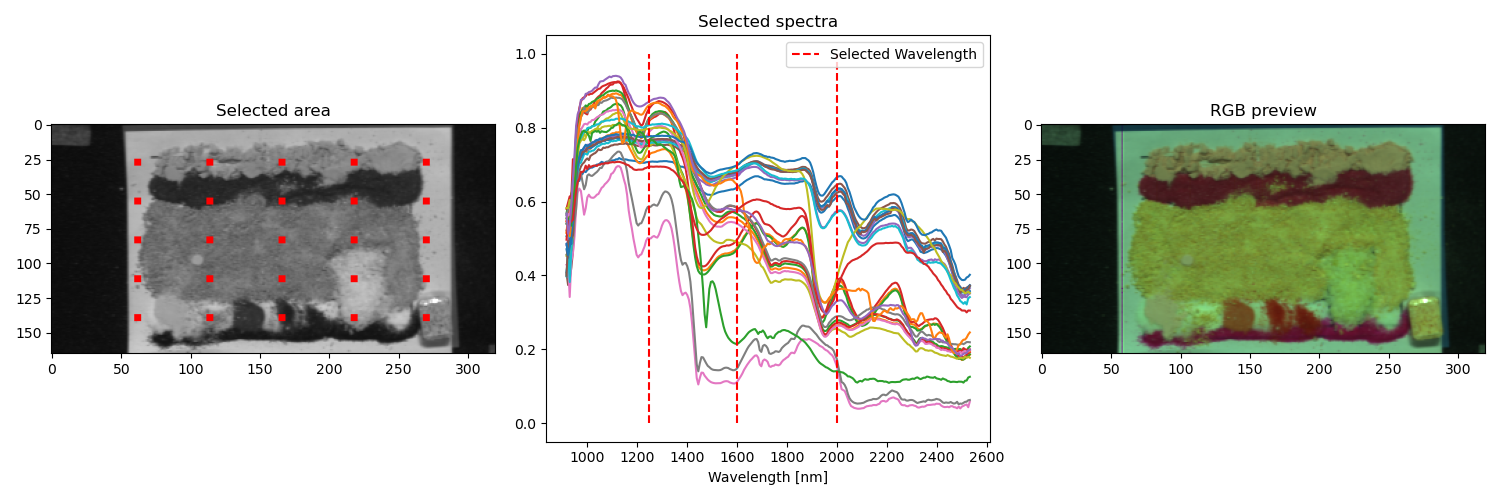
\includegraphics[width=0.8\textwidth]{./fig/task3/powder-segment.png}
  \caption{Segmentation results by Specim Scanner in infrared wavelengths}
  \label{fig:powder-seg}
\end{figure}
